\chapter{Opis projektnog zadatka}
		
		Velik broj kućnih ljubimaca iz raznih razloga odluta od svojih vlasnika. Jako ih je teško samostalno pronaći, pogotovo u velikim gradovima s mnogo ljudi i gustim prometom. Kako je nepraktično oglašavati njihove nestanke, opažanja i pronalaske s preciznim podacima putem uobičajenih internetskih platformi za komunikaciju koje nisu razvijene s ovom namjenom (npr. društvene mreže, stranice za oglašavanje i sl.), potrebno je razviti jednostavnu i korisnu aplikaciju koja će vlasnicima kućnih ljubimaca, skloništima za životinje, ali i drugim uključenim ljudima olakšati rješavanje ovih stresnih situacija. Tako će napokon svi podaci o nestancima, opažanjima i pronalascima biti okupljeni na jednome mjestu, umjesto kao do sada raspršeni. Osobi će pri pronalasku ili nestanku ljubimca obavještavanje ostalih brižnih vlasnika i drugih ljudi biti udaljeno samo nekoliko klikova. Naša aplikacija razvija se upravu u tu svrhu. U današnje vrijeme kad je tehnologija lako i široko dostupna, gotovo svi imaju mobilne uređaje pri ruci u svakom trenutku. Zato će aplikacija biti ciljano razvijena za mobilne uređaje, te će za sve dionike u ovom procesu podržavati što veću brzinu reagiranja, koja je često ključna za uspješan završetak potrage za kućnim ljubimcem. Nadamo se da će aplikacija pomoći ponovo ujediniti što je moguće više vlasnika s njihovim sretno pronađenim ljubimcima, te na jednom mjestu okupiti sve ljude koji su voljni pomoći u potragama. 

Slična aplikacija čije su slike dane kao primjer je američka aplikacija „MissingPetFinder“ koja je prilagođena korisnicima na njihovom području.  Njihova aplikacija ne nudi opciju skloništa, već je prilagođena isključivo za osobnu upotrebu. Također nudi dodatne opcije poput printanja letaka i slanja notifikacija koje za sada naša aplikacija ne nudi, iako je takva nadogradnja moguća ukoliko bi se pokazalo korisnim.

Aplikacija treba podržavati rad tri tipa korisnika:

		\begin{packed_item}
			
			\item  Neregistrirani korisnik
			\item  Registrirani korisnik
			\item  Sklonište
			
		\end{packed_item}

Pri otvaranju aplikacije korisniku se otvara opcija za prijavu u sustav, uz dodatne opcije registracije i ulaska kao gost.

		Prvi tip je \underbar{\textbf{neregistrirani korisnik}}. Pri ulasku u aplikaciju kao gost prikazuje mu se popis svih trenutno aktivnih oglasa o nestalim ljubimcima i osnovnim informacijama o njima (ime ljubimca, slike i broj mobitela vlasnika). Primjer sličnog rješenja nalazi se na slici ispod (slika \ref{fig:slika1}).

		%unos slike
		\begin{figure}[H]
			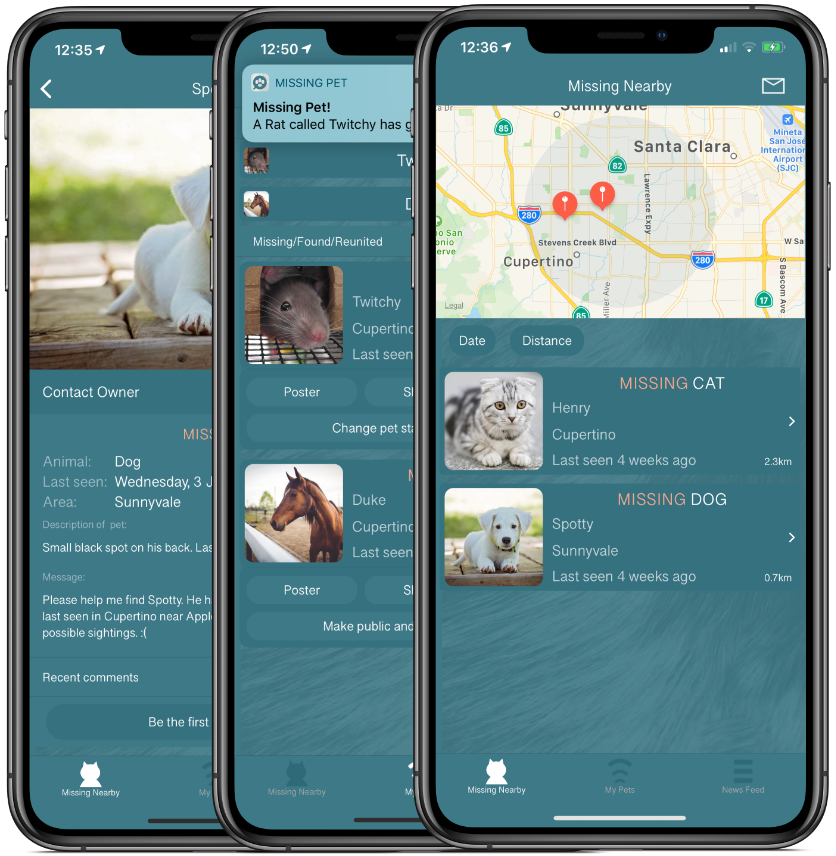
\includegraphics[scale=0.4]{slike/ljubimci.PNG} %veličina slike u odnosu na originalnu datoteku i pozicija slike
			\centering
			\caption{Primjer sličnog rješenja}
			\label{fig:slika1}
		\end{figure}

		Takav korisnik može i pretraživati oglašene nestale kućne ljubimce i skloništa za životinje. Pretraživanje je omogućeno po svim kategorijama podataka o ljubimcu koje su dostupne pri oglašavanju (osim slike i lokacije, vidi dolje), kao i po nazivu skloništa. Također, odabirom nekog od kućnih ljubimaca otvara se mogućnost detaljnijeg pregleda informacija o njemu (sve informacije unesene pri objavi oglasa) kao i pregled dosadašnje komunikacije oko potrage za ljubimcem.
Ako želi sudjelovati u potrazi za ljubimcem davanjem nekih informacija, neregistrirani korisnik se treba \underbar{registrirati}. Pri registraciji on unosi potrebne podatke kako bi kreirao svoj korisnički račun:

		\begin{packed_item}
			
			\item  Korisničko ime
			\item  Lozinka
			\item  Ime
			\item  Prezime
			\item  E-mail adresa
			\item  Broj mobitela
			
		\end{packed_item}

		Ako je uspješno unio sve podatke, registracija je uspješno provedena i korisnik je stvorio svoj profil u aplikaciji. U suprotnome će aplikacija zahtijevati ponovni unos podataka.

Drugi tip korisnika aplikacije je \underbar{\textbf{ registrirani korisnik}}. On je u prošlosti već stvorio svoj profil. Pri ulasku u aplikaciju on odabire opciju za prijavu te unosi svoje korisničko ime i lozinku. Uspješna prijava omogućuje mu pristup dodatnim stavkama ove aplikacije. Klikom na ikonu na \textit{toolbaru} može pregledati svoj profil. On, kao i neregistrirani korisnik ima opciju pregleda i pretraživanja oglasa, no njemu su pri pretraživanju dodatno dostupni ne samo aktivni, nego svi postojeći oglasi bez obzira koja im je kategorija oglasa postavljena. Osim ovih funkcija, nakon prijave korisnik također može i:

		\begin{packed_enum}
			
			\item  postaviti oglas o nestalom kućnom ljubimcu 
			\item  sudjelovati u komunikaciji oko potrage za ljubimcem 
			\item  ukloniti oglas o nestalom kućnom ljubimcu 
			\item  izmijeniti oglas o nestalom kućnom ljubimcu 
			
		\end{packed_enum}

		Takvom korisniku dostupna je opcija pregleda vlastitih oglasa. Kada ju odabere može pregledati sve oglase koje je on objavio, te mu postaju dostupne opcije za uklanjanje i izmjenu oglasa.

		Kada želi prijaviti nestanak ljubimca, korisnik odabire opciju postavljanja novog oglasa. \underbar{Postavljanje oglasa} uključuje unos sljedećih kategorija podataka:

		\begin{packed_item}
			
			\item  Vrsta
			\item  Ime na koje se odaziva
			\item  Datum i sat nestanka
			\item  Lokacija nestanka (bilježi se koristeći vanjsku uslugu za geolociranje)
			\item  Boja
			\item  Starost
			\item  Tekstni opis
			\item  Slika (maksimalno tri po oglasu)
			
		\end{packed_item}

		Oglas, osim ovih podataka, sadrži i kontakt podatke korisnika koji se automatski povlače iz korisničkih podataka danih pri registraciji (za običnog korisnika to su e-pošta i broj telefona, a dodatno za skloništa povlači se i naziv skloništa). Aplikacija pri unosu automatski provjerava je li korisnik unio sve podatke ispravno. Ako je unos ispravan, oglas je objavljuje i postaje dostupan svim korisnicima, a u protivnome se korisnik obavještava o grešci i od njega se traži ponovni upis podataka.

Kao i neregistrirani korisnik, nakon prijave korisnik može odabrati bilo koji oglas i klikom na njega dobiti više informacija o tom ljubimcu (slika \ref{fig:slika2}), kao i pregled dotadašnje komunikacije o potrazi. No, za razliku od neregistriranog, sada korisnik može i sudjelovati u komunikaciji ako misli da ima bilo kakvu korisnu informaciju (slika \ref{fig:slika3}). Komunikacija omogućuje unos tekstualne poruke (npr. obavijestiti vlasnika o pronalasku ili pojavi sličnog ljubimca, zatražiti više informacija ako nije siguran i slično), slike i slanje geolokacije (putem vanjske usluge, isto kao i kod postavljanja oglasa). Pri slanju bilo koje informacije aplikacija također automatski bilježi i kontakt podatke osobe koja informaciju šalje.

		\begin{figure}[H]
			\centering
			\begin{minipage}{.5\textwidth}
	 			 \centering
				  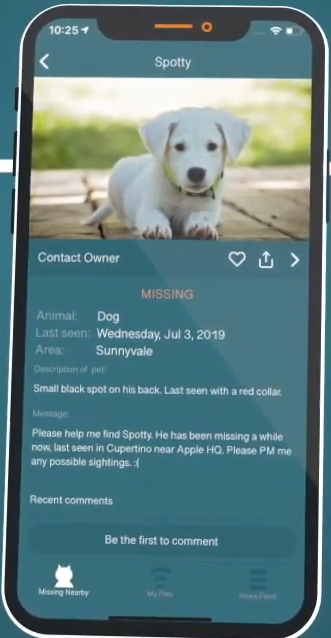
\includegraphics[width=.4\linewidth]{slike/viseInformacija.PNG}
				  \caption{Prikaz više informacija o ljubimcu kod sličnog rješenja}
				  \label{fig:slika2}
			\end{minipage}%
			\begin{minipage}{.5\textwidth}
				  \centering
				  
\includegraphics[width=.5\linewidth]{slike/Komunikacija.PNG}
				  \caption{Komunikacija kod sličnog rješenja}
				  \label{fig:slika3}
			\end{minipage}
		\end{figure}

		Iz bilo kojih razloga, korisnik uvijek ima mogućnost \underbar{ukloniti oglas} koji je sa svoga profila postavio. Uklanjanjem oglasa određeni oglas i sva njegova komunikacija nestati će iz popisa vidljivih oglasa, ali se oglas ne briše iz baze podataka. Tako on više neće biti dostupan ni njemu ni drugim korisnicima na pregled.

Registriranom korisniku nudi se i opcija izmjene oglasa koje je on postavio. \underbar{Izmjena oglasa} omogućuje izmjenu svih kategorija podataka o ljubimcu (navedeni gore kod postavljanja oglasa). Moguće je izmijeniti i kategoriju oglasa. Izbor kategorija oglasa uključuje:

		\begin{packed_enum}
			
			\item  Za ljubimcem se traga
			\item  Ljubimac je sretno pronađen
			\item  Ljubimac nije pronađen, ali je potraga obustavljena
			\item  Ljubimac je pronađen uz nesretne okolnosti
			
		\end{packed_enum}

		Po izvornim postavkama, pri objavi oglasa kategorija je automatski namještena da se za ljubimcem trenutno traga. Svaka izmjena kategorije oglasa u onu koja nije da se za ljubimcem aktivno traga automatski prebacuje oglas u popis neaktivnih oglasa, koji mogu pretraživati samo registrirani korisnici. 

Treći tip korisnika su \underbar{\textbf{skloništa za životinje}}. Skloništa za životinje su specijalni tip registriranih korisnika. Pri registraciji, kada se želi stvoriti profil za sklonište, potrebno je odabrati opciju „sklonište“. Unose se iste informacije kao i pri registraciji običnog korisnika, osim što se umjesto imena i prezimena osobe bilježi naziv skloništa. Prijava funkcionira isto kao i kod prijave običnih korisnika. U aplikaciji skloništa imaju dostupne sve opcije koje se nude i registriranim korisnicima (pregled i pretraživanje, postavljanje, uklanjanje i izmjena oglasa, te komunikacija oko potrage). Međutim, zbog toga što skloništa predstavljaju privremeni dom za mnoge tek pronađene ljubimce, kako bi se vlasnicima olakšalo lociranje njihovih ljubimaca, skloništa imaju i dodatnu mogućnost oglašavanja životinja koje su pronašli i koje se nalaze u njihovom prostoru. Zato skloništa pri postavljanju oglasa imaju ponuđenu i dodatnu opciju „u skloništu“ kojima tražene vlasnike obavještavaju da je ljubimac privremeno smješten kod njih, te čeka da vlasnici dođu po njega. Također, ako pronađu ljubimca čiji oglas već postoji, kada odaberu pregled detalja tog oglasa nudi im se opcija da označe da se taj ljubimac nalazi kod njih.

Ukoliko se aplikacija pokaže korisnom, nudi i brojne mogućnosti nadogradnje. Moguće bi bilo proširenje informacija koje se bilježe o ljubimcima, formiranje grupa za razgovor među vlasnicima koje bi mogle poslužiti i kao utjeha tijekom potrage za ljubimcima, dodavanje opcije videa, nagrada za pronalazak ljubimca ako vlasnik to želi, slanje obavijesti o nestancima u blizini i još mnogo drugih opcija.

		\eject
		
		